\chapter{REINFORCEMENT LEARNING}
\label{chap:rl_chap}

Machine Learning is the ability of a computer program that allows 
adaptation to new situations through experience, 
without explicitly programmed~\cite{mitchell_machine_1997}. 
As shown in \figref{fig:sl_ul_rl}, there exist three main paradigms: 

\textbf{Supervised Learning} is the task of learning a function $f \colon X \rightarrow Y$ 
that maps an input to an output based on $N$ example input-output pairs $(x_i,y_i)$ 
such that $ f(x_i) \approx y_i$, for all $i={1,2,...,N}$ 
by minimizing error between predicted and target output. 
Input $x$ can be thought as the state of an agent, and $y$ is the correct action at state $x$. 
For supervised learning, both $x$ and $y$ should be available, 
where the correct actions are provided by a friendly supervisor~\cite{russell_artificial_nodate}. 

\textbf{Unsupervised Learning} discovers the structure on input examples without any label on them. 
Based on $N$ example input $(x_i)$, 
it discovers function $f \colon X \rightarrow Y$, $ f(x_i) = y_i$, for all $i={1,2,...,N} $, 
where $y_i$ is discovered output. 
This discovery is motivated by predefined objective. 
This objective is maximization of a value which represents compactness of output representations. 
Again, input $x$ can be thought as the state of an agent. 
However, correct action is not available and there is no given hint in this case. 
It can learn relations among states but it does not know what to do 
since there is no target or utility~\cite{russell_artificial_nodate}.
 
\textbf{Reinforcement Learning} is one of the three main machine learning paradigms along with Supervised and Unsupervised Learning. 
It is the closest kind of learning demonstrated by humans and animals 
since it is grounded by biological learning systems. 
It is based on maximizing cumulative reward over time to make agent 
learn how to act in an environment~\cite{sutton_reinforcement_1998}. 
Each action of the agent is either rewarded or punished according to a reward function. 
Therefore, reward function is mathematical representation of what to teach the agent. 
The agent explores environment by taking various actions in different states to gain experience, based on trial-and-error. 
Then it exploits experiences to get the highest reward from the environment considering instant and future rewards over time. 

Formally, Reinforcement Learning is learning a policy function 
$\pi \colon \mathcal{S} \rightarrow \mathcal{A}$ which maps 
inputs (observations) $s \in \mathcal{S}$ to outputs (actions) $a \in \mathcal{A}$. 
Learning is achieved by maximization of the value function $V^{\pi}(s)$ (cumulative reward) for all possible states, which depends on policy $\pi$. 
In this sense, it is similar to unsupervised learning. 
However, the difference is that the value function $V^{\pi}(s)$ is not defined exactly unlike unsupervised learning setting. 
It is also learned by interacting with the environment by taking all possible actions in all possible states. 

In short, Reinforcement Learning is different from Supervised Learning because the correct actions are not provided. 
It is also different from Unsupervised Learning because the agent is forced to learn a specific behaviour and evaluated at each time step without supervision. 

\begin{figure}
	\centering
	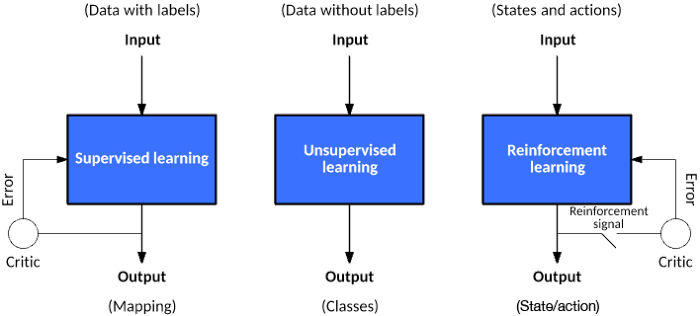
\includegraphics[width=0.95\textwidth]{figures/ml_theory/sl_ul_rl.png}
	\caption{Main paradigms of ML \cite{noauthor_models_nodate}}
	\label{fig:sl_ul_rl}
\end{figure}

